 % !TEX root = Stanfill_CoDA.tex
\section{Results}\label{sec:results}

In this section we summarize and present the main findings of the simulation study for  estimating the central direction $\bm S = \bm I_{3\times 3}$ with the four proposed estimators of Section~\ref{sec:estimators}. We quantify the estimation error between the true location $\bm S = \bm I_{3\times 3}$ and an estimate $\widehat{\bm S}$ using the geodesic distance, i.e.  
\begin{equation}
\Rdist(\bm{S}, \widehat{\bm{S}}) =  \frac{1}{\sqrt{2}}||
\Log(\bm{S}^\top\widehat{\bm{S}})||_F, \quad \mbox{where} \quad \widehat{\bm{S}} =  \ProjMean, \; \GeomMean,\;  \ProjMedian \; \mbox{or} \; \GeomMedian.
\end{equation}

\noindent Note that for any two rotations $\bm R_1$ and $\bm R_2$ in $SO(3)$ it holds that their Euclidean distance $\Edist(\bm R_1,\bm R_2)=2\sqrt{2}\sin[\Rdist(\bm R_1,\bm R_2)/2]$. We refer to Section~\ref{sec:appendix2} of the Appendix for a short proof of this result.  Hence, results using $\Edist$ would prove equivalent, albeit on a smaller scale.   
%\begin{center}
\begin{figure}[h!]
\centering
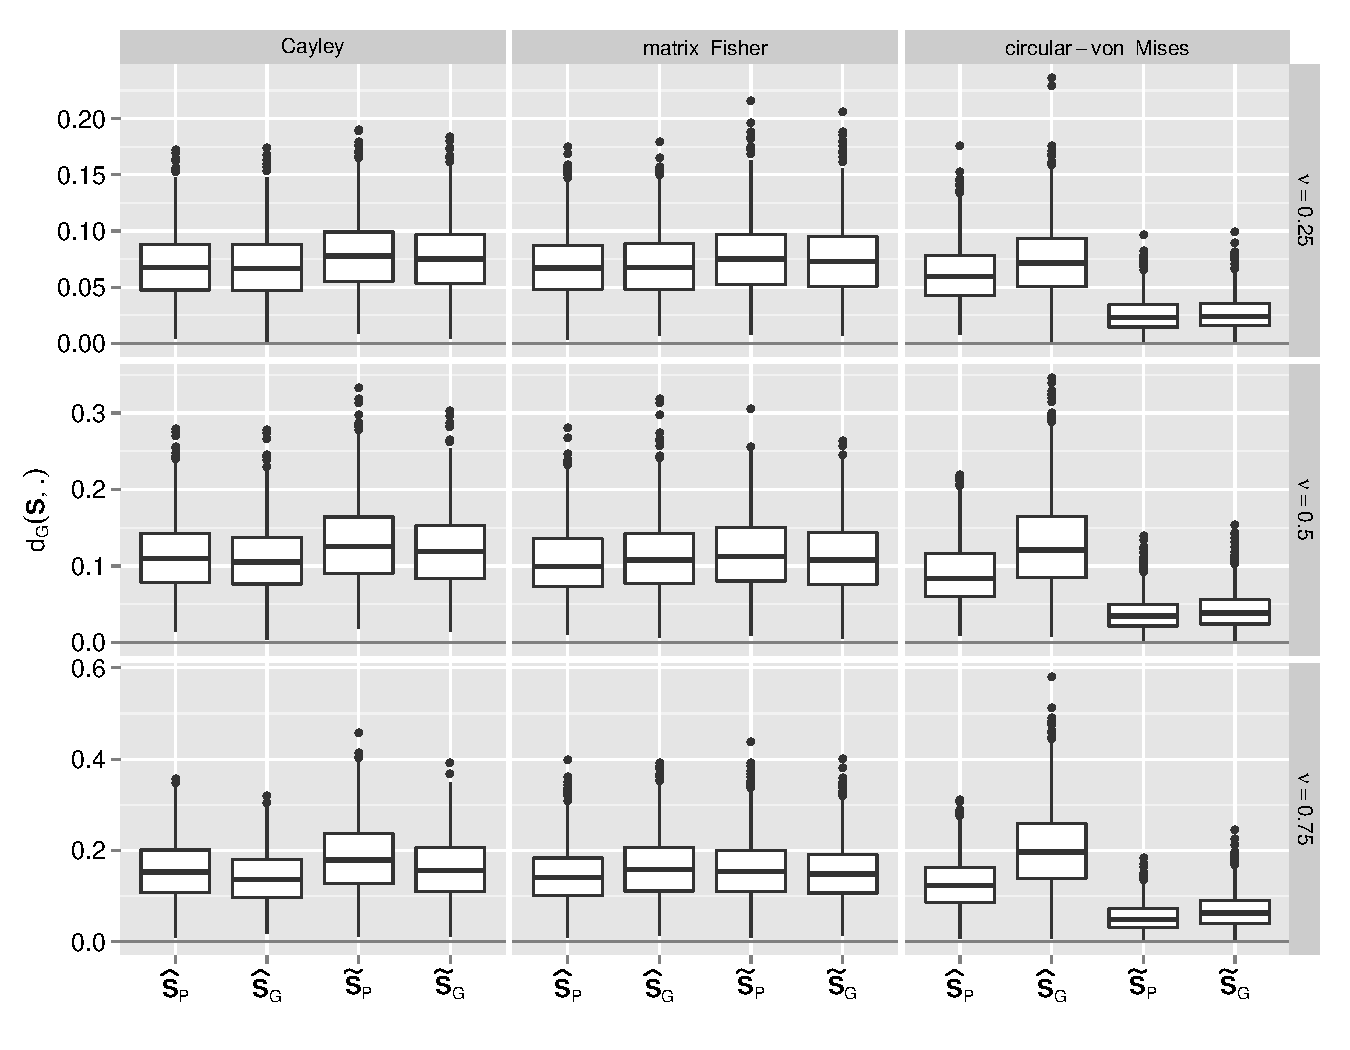
\includegraphics[width=0.8\textwidth]{N100AllNuBoxes.pdf}
\caption{Boxplots of the estimation errors for each rotation distribution and level of $\nu$,  $n=100$.}
\label{fig:NuBoxes}
\end{figure}
%\end{center}
Figure~\ref{fig:NuBoxes} displays side-by-side boxplots showing the estimation errors of all four estimators for a given choice of rotation distribution and circular spread $\nu$ when  $n=100$.  For a tabular summary of this figure including the root mean square error (RMSE) as a measure of precision as well as the \textit{mean estimation error} refer to Table \ref{tab:alldN100} in Section~\ref{sec:appendix3} of the Appendix. Despite skewness in some of the plotted error distributions the \textit{median estimation error} was quantitatively similar to the mean estimation error and is therefore not reported.

First and foremost the results suggest that different location estimators emerge as preferable depending on the type of distribution assumed for the rotation errors in \eqref{eqn:1}.  For the circular-von Mises-based distribution both median-type estimators ($\ProjMedian$ and $\GeomMedian$) are superior with respect to the estimation error while for the Cayley and matrix Fisher models the mean-type estimators ($\ProjMean$ and $\GeomMean$) perform better though on less pronounced scale.  While preferences within the median- and mean-type estimators are visible, these generally disappear as the variability in the data, i.e.~$\nu$ decreases.  For the Cayley and the matrix Fisher distribution the overall pattern of estimation is similar. $\ProjMean$ and $\GeomMean$ typically exhibit less spread and a lower average estimation error than $\ProjMedian$ and $\GeomMedian$ but differences between the estimators lessen as $\nu$ becomes smaller. Figure~\ref{fig:NuBoxes} further shows that the estimation error is a function of the circular spread $\nu$; as $\nu$ decreases the range of the observed estimation errors decreases within each rotation model and for each of the four estimators. The same is true for the mean estimation error, and RMSE as indicated Table~\ref{tab:alldN100} in Section~\ref{sec:appendix3} of the Appendix.  Figure~\ref{fig:NBoxes}, also in Section~\ref{sec:appendix2} of the Appendix, is a graphic similar to Figure~\ref{fig:NuBoxes} in which the estimation errors are given as a function of sample size for $\nu=0.75$.

%\begin{center}
%\begin{table}[h!]
%\caption{Numerical summaries of the estimation error  by distribution, $n=100$,  $\nu=0.25$.  \label{tab:alldN100Nu25}}
%\begin{tabular}{ccccccccccc}
%  \hline
%		& &\multicolumn{3}{c}{\textbf{Cayley}} & \multicolumn{3}{c}{\textbf{matrix Fisher}}  & \multicolumn{3}{c}{\textbf{circular-von Mises}}\\ 
%Estimator 	& &  Mean error & RMSE& &  Mean error & RMSE& &   Mean error & RMSE \\  \hline \hline %\rule[2mm]{0mm}{3mm} 
% 		  $\GeomMean$ & &  0.069 & 0.075 & &  0.070 & 0.076&  & 0.074 & 0.081 \\ 
% 		 $\ProjMean$ &  & 0.070 & 0.076 & &  0.070 & 0.076&  &  0.062 & 0.067\\ 
%		 $\GeomMedian$ &  & 0.077 & 0.083 & &  0.075 & 0.081&  & 0.027 & 0.031\\ 
% 		  $\ProjMedian$ &  & 0.079 & 0.086 & &  0.077 & 0.083 & & 0.026 & 0.030\\ \hline
%\end{tabular}
%\end{table}
%\end{center}

%\begin{table}[h!]
%\centering
%\footnotesize
%\caption{Numerical summaries of the estimation error  by distribution, $n=100$,  $\nu=0.25$ and $0.75$.  \label{tab:alldN100Nu25}}
%\begin{tabular}{cccccccccccc}
%\hline
%& &\multicolumn{3}{c}{\textbf{Cayley}} & \multicolumn{3}{c}{\textbf{matrix Fisher}}  & \multicolumn{3}{c}{\textbf{circular-von Mises}}\\ 
%  \hline
% $\nu$ & Estimator && Mean error (SE) & RMSE && Mean error (SE) & RMSE && Mean error (SE) & RMSE \\ 
%  \hline
% \multirow{4}{*}{0.25} & $\GeomMean$ && 0.0690 (0.0009) & 0.0752 && 0.0699 (0.0010) & 0.0761 && 0.0744 (0.0010) & 0.0811 \\ 
%   & $\ProjMean$ && 0.0698 (0.0009) & 0.0759 && 0.0695 (0.0009) & 0.0756 && 0.0617 (0.0008) & 0.0671 \\ 
%    & $\GeomMedian$&& 0.0769 (0.0010) & 0.0834 && 0.0747 (0.0010) & 0.0813 && 0.0269 (0.0005) & 0.0310 \\ 
%    & $\ProjMedian$ && 0.0791 (0.0011) & 0.0858 && 0.0766 (0.0010) & 0.0832 && 0.0256 (0.0005) & 0.0296 \\ \hline
%   \multirow{4}{*}{0.75} & $\GeomMean$ && 0.1398 (0.0018) & 0.1514 && 0.1703 (0.0045) & 0.2225 && 0.2039 (0.0028) & 0.2221 \\ 
%    & $\ProjMean$ && 0.1567 (0.0020) & 0.1695 && 0.1462 (0.0020) & 0.1588 && 0.1276 (0.0017) & 0.1388 \\ 
%    & $\GeomMedian$ && 0.1597 (0.0021) & 0.1729 && 0.1527 (0.0021) & 0.1660 && 0.0687 (0.0012) & 0.0792 \\ 
%    & $\ProjMedian$ && 0.1847 (0.0024) & 0.2000 && 0.1597 (0.0022) & 0.1736 && 0.0547 (0.0010) & 0.0628 \\ 
%   \hline
%\end{tabular}
%\end{table}

%\begin{figure}[h!]
%\centering
%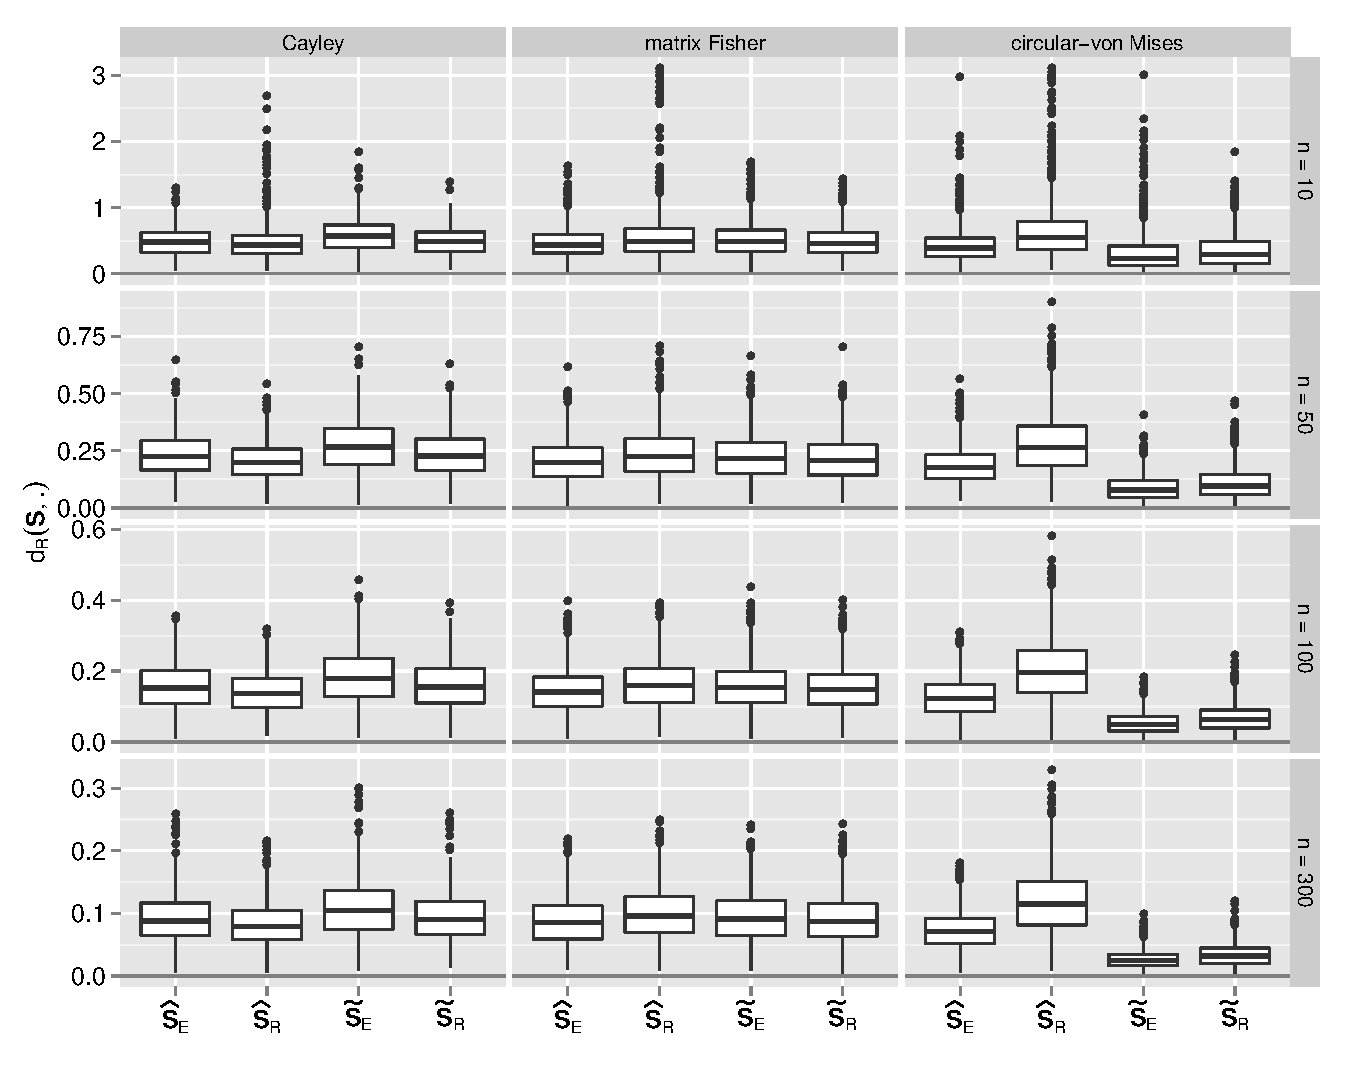
\includegraphics[width=1\textwidth]{Nu75AllNBoxes.pdf}
%\caption{Box-plots of the estimation error for each rotation distribution and level of $n$,  $\nu=0.75$.}
%\label{fig:NBoxes}
%\end{figure}

%Figure \ref{fig:NBoxes} illustrates the behavior of the estimators as a function of the sample size. Results are displayed for each level of $n$ for  $\nu=0.75$. As to be expected, the estimation error decreases as the sample size increases for all three distributions. For small samples, $n=10$, the estimator exhibiting the largest amount of variability is the geodesic mean $\GeomMean$. This behavior is consistent for all three distributions.  While the estimator's variability lessens considerably for the Cayley and matrix Fisher distribution as $n$ increases, the estimator remains the most variable estimator for the circular-von Mises-based distribution.  A possible explanation for this behavior is that the algorithm to estimate $\GeomMean$ uses a random sample point in its initiating step.  For small samples or samples with several extreme observations it is likely to start the algorithm far from the true center, which in turn may cause the algorithm to get stuck in a local minimum and to fail to converge globally.  In practice we suggest the algorithm be started at some other location estimate of $\bm S$, e.g.~ at $\ProjMean$. In simulations where $\ProjMean$ was used as a starting point for the algorithm we observed  similar results with less variability in the estimates of $\GeomMean$ but for the purpose of a fair comparison we started the algorithm at a random sample point.  We refer to Figure \ref{fig:vmnu75} for a comparison of all estimators for the circular-von Mises-based distribution case when $\nu=0.75$.  

%\begin{center}
%\begin{table}[h!]
%\caption{Numerical summaries of the estimation error for all levels of $n$ for the circular-von Mises-based distribution,  $\nu=0.75$.  \label{tab:vmnu75}}
%\begin{tabular}{rccccrccc}
%  \hline
% $\mathbf{n}$ & \textbf{Estimator}  & \textbf{Mean error} & \textbf{RMSE} & &$\mathbf{n}$ & \textbf{Estimator} & \textbf{Mean error} & \textbf{RMSE} \\ \hline \hline
%   \multirow{4}{*}{10} & $\GeomMean$  & 0.652 & 0.789 &  & \multirow{4}{*}{100} & $\GeomMean$  & 0.204 & 0.222 \\ 
%    & $\ProjMean$  & 0.442 & 0.518 &   & & $\ProjMean$ & 0.128 & 0.139 \\ 
%    & $\GeomMedian$  & 0.366 & 0.459 &  &  & $\GeomMedian$  & 0.069 & 0.079 \\ 
%    & $\ProjMedian$  & 0.326 & 0.450 &   & & $\ProjMedian$  & 0.055 & 0.063 \\  
%    & & & & & & & \\ 
%    \multirow{4}{*}{50} & $\GeomMean$  & 0.280 & 0.309 &  &  \multirow{4}{*}{300} & $\GeomMean$  & 0.119 & 0.130 \\ 
%    & $\ProjMean$  & 0.185 & 0.202 &  &  & $\ProjMean$  & 0.075 & 0.081 \\ 
%    & $\GeomMedian$  & 0.109 & 0.130 &  & & $\GeomMedian$  & 0.034 & 0.039 \\
%    & $\ProjMedian$ & 0.088 & 0.105 &  &  & $\ProjMedian$ & 0.027 & 0.031 \\ 
%   \hline
%\end{tabular}
%\end{table}
%\end{center}

\begin{figure}[h!]
\centering
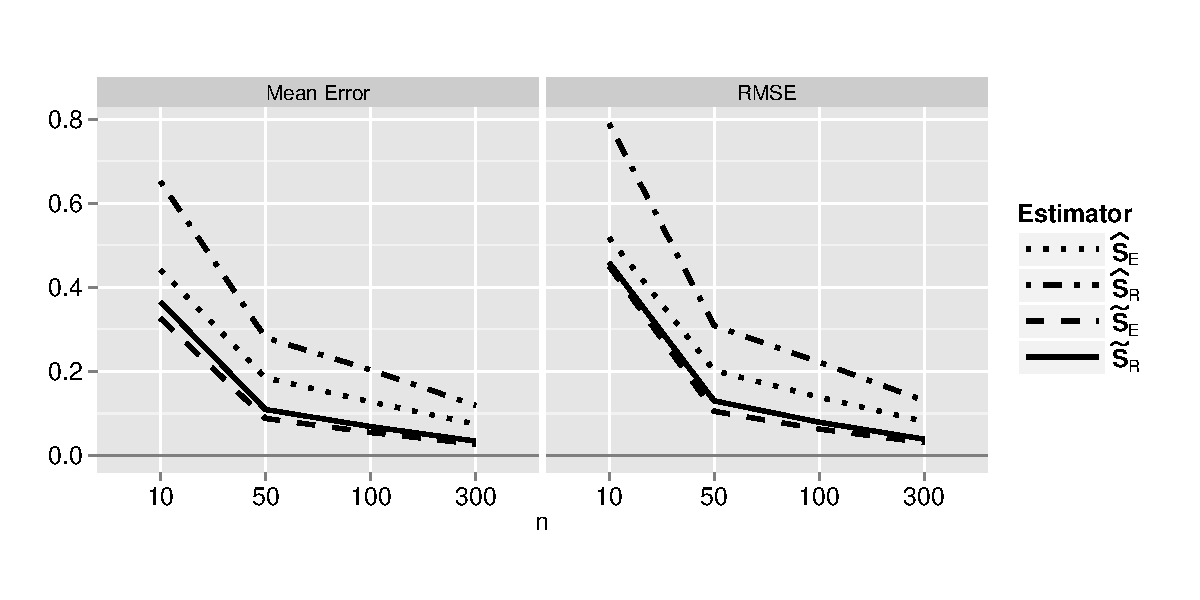
\includegraphics[width=0.8\linewidth]{vonMisesnu75MeanRMSE.pdf}
\caption{Plot of the estimation error for all levels of $n$ for the circular-von Mises-based distribution,  $\nu=0.75$.}  \label{fig:vmnu75}
\end{figure}

To explore the results for the circular-von Mises-based distribution further see Figure~\ref{fig:vmnu75}, which depicts the mean estimation error and RMSE as a function of sample size for $\nu=0.75$.  Here we see more clearly that the median estimators are preferred over the mean estimators for all sample sizes.  Figure \ref{fig:denzoom} may provide an explanation for why the circular-von Mises-based distribution so clearly distinguishes between the mean- and median-type estimators.  Upon closer examination of the tail of all three rotation densities (expressed in terms of the misorientation angle $r$ as in Figure~\ref{fig:Haar}) the circular-von Mises-based distribution exhibits the heaviest tail with respect to the Haar measure. As a consequence, \textit{more extreme} observations are more likely to be sampled under the circular-von Mises-based distribution compared to the Cayley and matrix Fisher models suggesting that a median-type estimator is more favorable. 

% \begin{figure}[h!]
% \centering
% \subfloat[$\nu=0.75$]{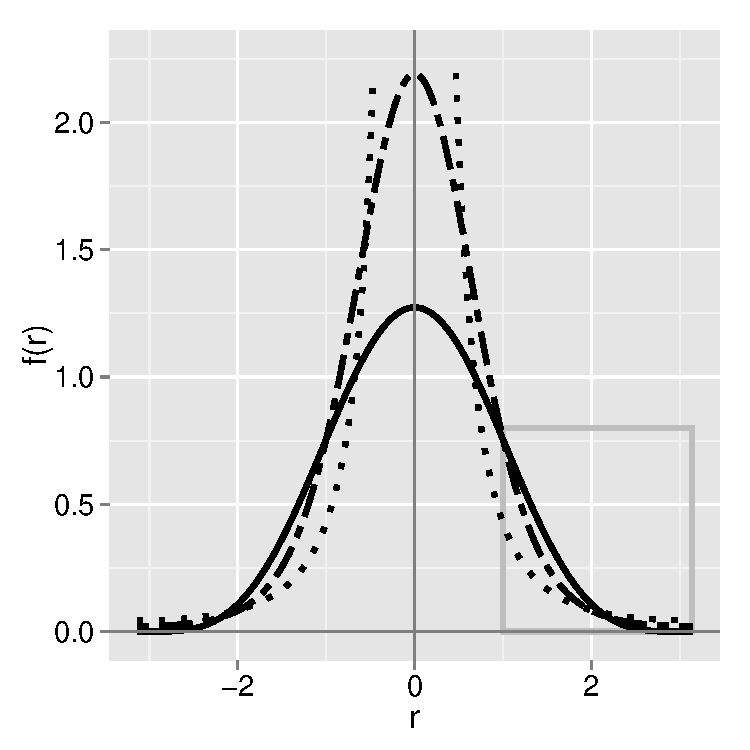
\includegraphics[width=.45\textwidth]{Var75DensityBox}}
% \subfloat[Detail]{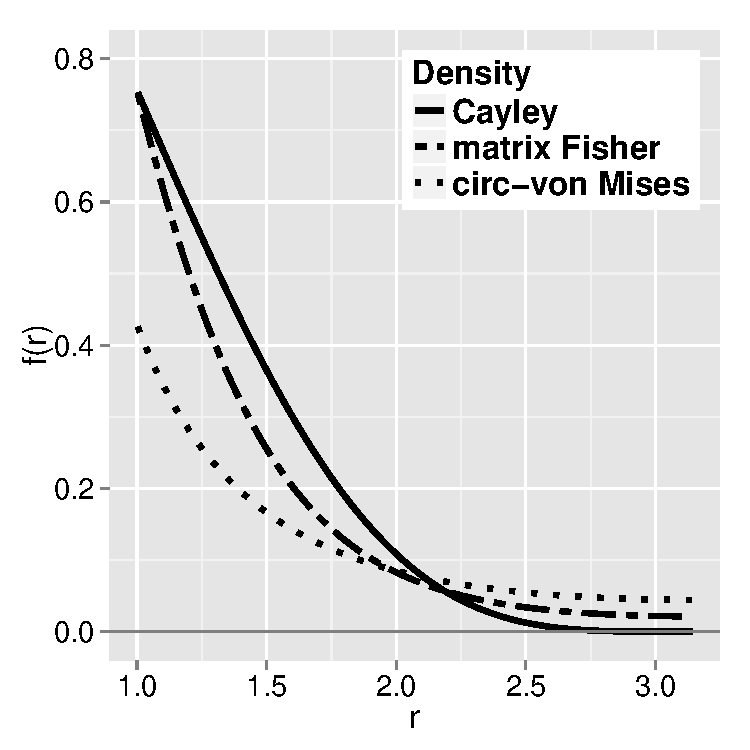
\includegraphics[width=.45\textwidth]{Var75DensityZoom}}
% \caption{Angular densities under consideration; $\nu=0.75$ (a) and tail behavior (b) }
% \label{fig:dendetail}
% \end{figure}

We use Figure \ref{fig:SimTail} to examine the  extent to which the tail-behavior accounts for the observed differences in the mean- and median-type estimators. Figure \ref{fig:SimTail} displays the tail weight for each sample (i.e.~the proportion of observations in the sample considered to come from the tail of the distribution) plotted against the difference in errors for the mean- and median-type estimators.  The results shown in Figure \ref{fig:SimTail} are with respect to the Euclidean geometry-based estimators $\ProjMean$ and $\ProjMedian$. Similar results are obtained for the Riemannian geometry-based estimators $\GeomMean$ and $\GeomMedian$ and therefore are omitted. Note that we define the tail to be the average crossing point at which the distributions cross for the second time, see Figure~\ref{fig:denzoom}. From  Figure \ref{fig:SimTail} we can see that in general there appears to be a positive relationship between the proportion of observations in the tail and the relative difference in estimator error indicating that with increasing tail weight the error of the mean estimator indeed increases at a higher rate than does the error of the median estimator. That is, as the tail becomes heavier the projected median is preferable to the projected mean more often.  Values on the $y$-axis not only indicate the preferred estimator, but also the magnitude of the preference.  For example, a $y$-value of 0 suggests that the two estimators result in equivalent estimates in terms of their distance from the true $\bm S$.  The more extreme a $y$-value is in the negative direction, e.g.~close to $-0.5$ and beyond, the closer the projected-mean is to the truth in comparison to the projected median. At $-0.5$ the error associated with the projected median is three times that of the projected mean.  Likewise,  large positive $y$-values around $1$ signify that the error by the projected median is roughly zero compared to the error of the projected median.


\begin{figure}[h!]
\centering
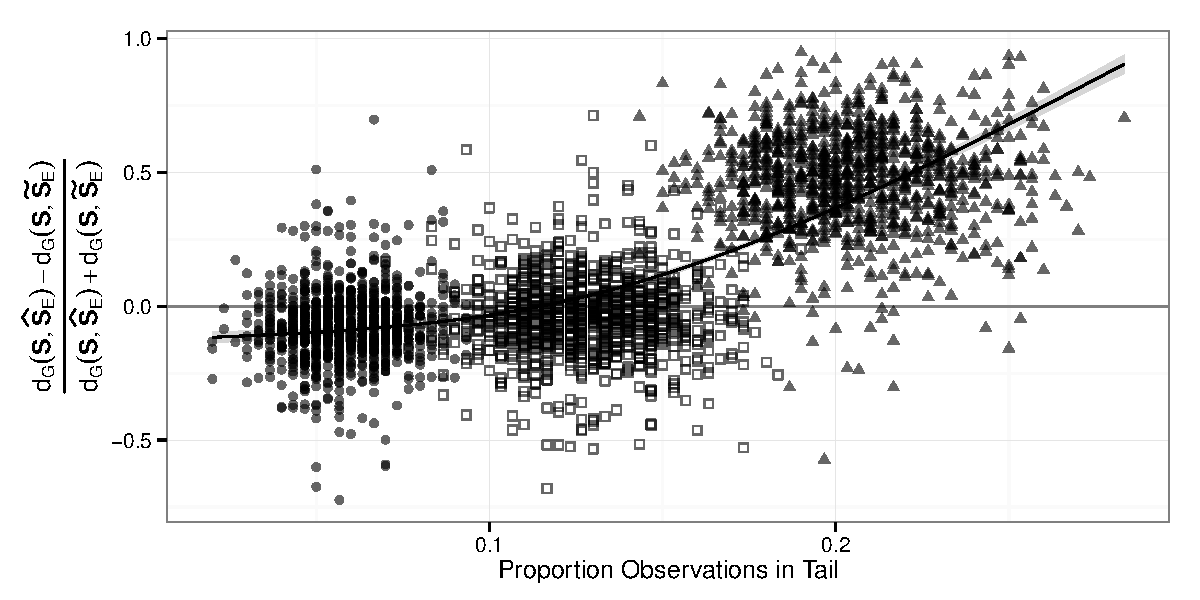
\includegraphics[width=.8\textwidth]{Nu75N300TailBehaviorStandard}
\caption{The proportion of observations in the tail against the difference in projected mean and median errors for simulated data with $n=300$.  Different symbols indicate different error distributions.}
\label{fig:SimTail}
\end{figure}

We next explore the effect the choice of geometry, i.e.~Riemannian vs.~Euclidean, has on the estimation error for both types of loss functions. To provide more insight into possible differences we plot the estimation error resulting from $\Edist$ ($x$-axis) versus the estimation error resulting from $\Rdist$ ($y$-axis) for $n=100$ and $\nu=.25$,  $\nu=.75$, respectively; see~Figures~\ref{fig:comPL2} (a) and (b).   
Mean-type estimators are represented by black dots whereas median-type estimators correspond to light gray dots. A point falls below the $45^\circ{}$ line if the error on the $y$-axis corresponding to the Riemannian geometry-based estimator is smaller in comparison to the error plotted on the $x$-axis for the Euclidean geometry-based estimator.  The same holds true in the opposite direction if a point falls above the $45^\circ{}$ line. 
For example, in Figure \ref{fig:comPL2},  $\GeomMedian$ tends to yield less estimation error than $\ProjMedian$  for the Cayley distribution as most of the points fall below the identity line while the Riemannian distance-based $\GeomMedian$ results in greater errors for ${\bm S}$ for the circular-von Mises-based distribution.  This conclusion supports results for $\ProjMedian$ and $\GeomMedian$ seen in Figure~\ref{fig:NuBoxes}.

\begin{figure}[h!]
\centering
\subfloat{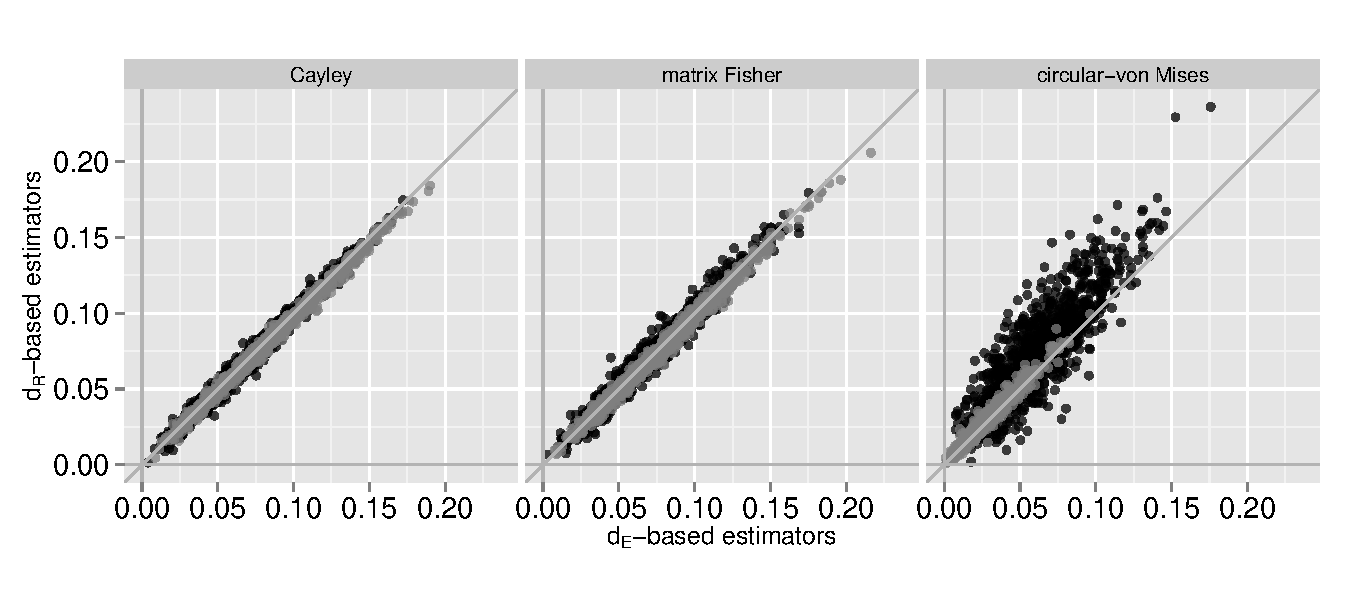
\includegraphics[width=0.8\linewidth]{EuclidRiemannNu25.pdf}}\\
\subfloat{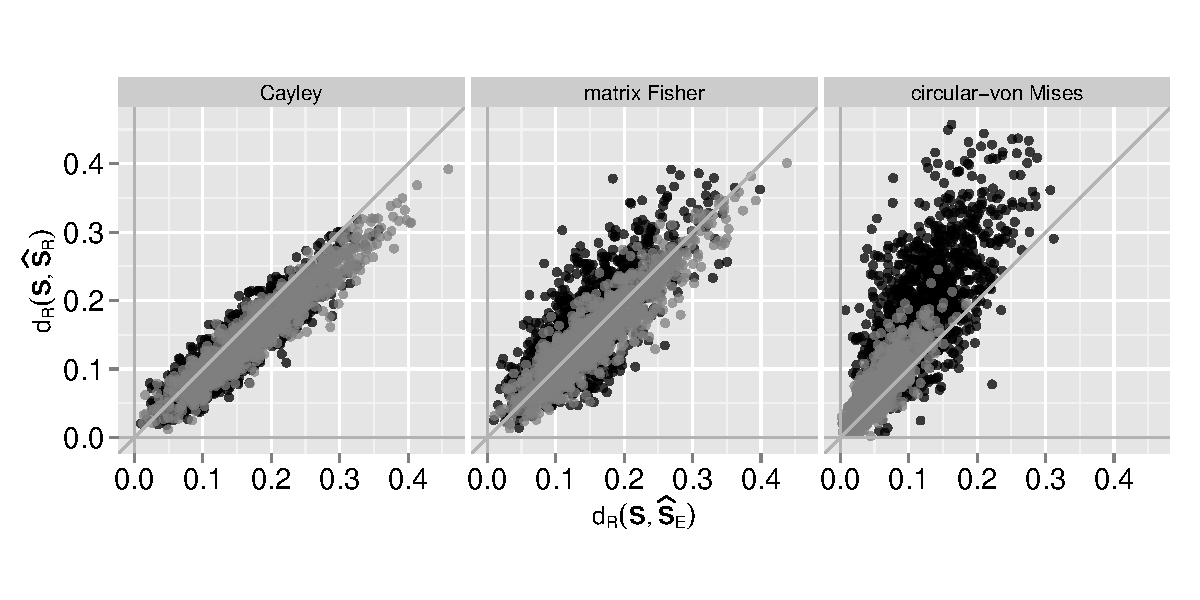
\includegraphics[width=0.8\linewidth]{EuclidRiemannNu75.pdf}}
\caption{Comparison of the estimation errors resulting from the embedding ($x$-axis) and intrinsic ($y$-axis) approaches, $n=100$.  The mean-type estimators are in black dots and the median-type estimators are in light gray.}
\label{fig:comPL2}
\end{figure}

%\begin{table}[h]
%\caption{Average reduction in estimation error by using $\GeomMedian$ instead of $\ProjMedian$, $\delta=\Rdist(\ProjMedian,\bm S) - \Rdist(\GeomMedian,\bm S)$ and percentage of samples for which $\Rdist(\GeomMedian,\bm S) < \Rdist(\ProjMedian,\bm S)$.}
%\label{tab:percL1}
%\begin{center}
%\footnotesize
%\begin{tabular}{rrcrrcrrcrr}
%  \hline
%  & &&\multicolumn{2}{c}{\textbf{Cayley}} & &\multicolumn{2}{c}{\textbf{matrix} } &&\multicolumn{2}{c}{\textbf{circular-}}\\
%    && &\multicolumn{2}{c}{} & &\multicolumn{2}{c}{\textbf{Fisher}} & &\multicolumn{2}{c}{\textbf{von Mises}}\\ 
%\rule[2mm]{0mm}{3mm} 
%  &  $n$ && $\bar{\delta}$ & \% & & $\bar{\delta}$ & \% & & $\bar{\delta}$ & \% \\ 
%  \hline \hline
%  \multirow{4}{*}{$\nu=0.25$} 
%  &   10 & & 0.008 & 0.743 & &  0.006 & 0.725 & & -0.005 & 0.328 \\ 
%  &   50 & &  0.003 & 0.783 & &  0.002 & 0.697 & & -0.002 & 0.327 \\ 
%  &  100 & &  0.002 & 0.789 & & 0.002 & 0.712 & & -0.001 & 0.308 \\ 
%  &  300 & & 0.001 & 0.781 & & 0.001 & 0.711 & & -0.001 & 0.284 \\ \hline
%  \multirow{4}{*}{$\nu=0.50$} 
%   &   10 & & 0.031 & 0.772 & &  0.017 & 0.662 & &  -0.019 & 0.335 \\ 
%   &   50 & & 0.013 & 0.811 & & 0.005 & 0.620 & &-0.008 & 0.282 \\ 
%   &  100 & & 0.009 & 0.809 & &  0.005 & 0.660 & &  -0.005 & 0.302 \\ 
%   &  300 & & 0.005 & 0.804 & &  0.002 & 0.658 & & -0.003 & 0.255 \\ \hline
%   \multirow{4}{*}{$\nu=0.75$} 
%  &  10 & & 0.089 & 0.821 & & 0.034 & 0.633 & & -0.040 & 0.322 \\ 
%  &   50 & & 0.037 & 0.866 & & 0.009 & 0.597 & & -0.021 & 0.238 \\ 
%  &  100 & &  0.025 & 0.858 & & 0.007 & 0.603 & & -0.014 & 0.240 \\ 
%  &  300 & &  0.014 & 0.850 &&  0.003 & 0.589 & & -0.007 & 0.218 \\ 
%   \hline
%\end{tabular}
%\end{center}
%\end{table}

In Tables \ref{tab:percL1} and \ref{tab:percL2} of Section~\ref{sec:appendix3} of the Appendix we support Figure~\ref{fig:comPL2} with an exact count (expressed as a percentage) of how often $\Rdist$ resulted in a smaller estimation error than $\Edist$.  Additionally, we show the average amount by which the $\Rdist-$ and $\Edist-$based estimates deviate from one another.  %We denote the latter quantity by $\bar\delta$ in Table \ref{tab:percL1} where  $\delta=\Rdist(\ProjMedian,\bm S)-\Rdist(\GeomMedian,\bm S)$.    
Our previous results suggested the use of median-type estimators for the circular-von Mises-based distribution which favors $\ProjMedian$ over $\GeomMedian$ as $\Rdist(\ProjMedian,\bm S) < \Rdist(\GeomMedian,\bm S)$ most of the time.  For the Cayley and the matrix Fisher model the preference is reversed, typically  $\ProjMedian$ exhibits a larger spread (cf.~Figure~\ref{fig:NuBoxes}). 


%\begin{table}[h!]
%\caption{Average reduction in estimation error by using $\GeomMean$ instead of $\ProjMean$, $\delta=\Rdist(\ProjMean,\bm S) - \Rdist(\GeomMean,\bm S)$ and percentage of samples for which $\Rdist(\GeomMean,\bm S) < \Rdist(\ProjMean,\bm S)$.  \label{tab:percL2}}
%\begin{center}
%\footnotesize
%\begin{tabular}{rrcrrcrrcrr}
%  \hline
%  & &&\multicolumn{2}{c}{\textbf{Cayley}} & &\multicolumn{2}{c}{\textbf{matrix} } &&\multicolumn{2}{c}{\textbf{circular-}}\\
%    && &\multicolumn{2}{c}{} & &\multicolumn{2}{c}{\textbf{Fisher}} & &\multicolumn{2}{c}{\textbf{von Mises}}\\ 
%\rule[2mm]{0mm}{3mm} 
%  &  $n$ && $\bar{\delta}$ & \% & & $\bar{\delta}$ & \% & & $\bar{\delta}$ & \% \\ 
%  \hline \hline
%\multirow{4}{*}{$\nu=0.25$}
%  &   10 &&  0.001 & 0.521 &&  -0.002 & 0.450 && -0.034 & 0.128 \\  
%  &   50 && 0.001 & 0.531 &&  -0.001 & 0.435 && -0.016 & 0.209 \\\ 
%  &  100 && 0.001 & 0.565 &&  -0.000 & 0.469 && -0.013 & 0.201 \\
%  &  300 && 0.000 & 0.588 &&  -0.000 & 0.486 &&  -0.007 & 0.239 \\ \hline
%  \multirow{4}{*}{$\nu=0.50$}
%   &   10 &&   0.010 & 0.592 &&  -0.018 & 0.434 &&  -0.101 & 0.157 \\ 
%   &   50 &&  0.007 & 0.645 &&  -0.011 & 0.392 &&  -0.055 & 0.145 \\ 
%   &  100 &&   0.004 & 0.642 &&  -0.007 & 0.393 &&  -0.038 & 0.162 \\ 
%   &  300 &&   0.003 & 0.642 &&  -0.004 & 0.393 &&  -0.023 & 0.157 \\ \hline
%  \multirow{4}{*}{$\nu=0.75$}
%   &   10 &&   0.016 & 0.668 &&  -0.096 & 0.357 &&  -0.210 & 0.171 \\ 
%   &   50 &&  0.026 & 0.741 &&  -0.036 & 0.338 &&  -0.096 & 0.150 \\
%   &  100 &&  0.017 & 0.735 &&  -0.024 & 0.346 &&  -0.076 & 0.111 \\ 
%   &  300 &&  0.009 & 0.728 &&  -0.012 & 0.344 && -0.045 & 0.127 \\ 
%   \hline
%\end{tabular}
%\end{center}
%\end{table}

Similarly to the median-type estimators, $\Rdist$ is the preferred metric for the Cayley distribution especially when $\nu$ is large.  For the  matrix Fisher distribution the preference is less clear, especially for less variable data, but as $\nu$ increases the Euclidean-based mean yields generally a smaller estimation error more often. In summary,
\begin{itemize}
\item the choice of location estimator can depend on the rotation error distribution in the location model (1).  For the matrix Fisher and the Cayley distribution  the projected arithmetic mean $\ProjMean$ and the geometric mean $\GeomMean$ are, respectively, preferable though $\ProjMedian$ and $\GeomMedian$ are not far behind especially when the circular spread is smaller. For the circular-von Mises-based distribution  the projected median $\ProjMedian$  should be used.

\item  However, a significant finding of these simulation results is that the (Euclidean-based)  projected median $\ProjMedian$ is typically a good location estimator across rotation error models.  For the circular-von Mises-based estimation, this generally has the best performance, while for the Cayley or matrix Fisher distributions, this estimator is often quite comparable to the best estimator.  In other words, an estimator $\ProjMedian$ not previously considered for rotation matrices in the literature appears to be suggestible, particularly in small samples and without knowledge of the underlying rotation error distribution.

\end{itemize}